\documentclass[10pt]{beamer}
\usetheme{Madrid}
\setbeamercovered{dynamic}
\setbeamertemplate{navigation symbols}{}

\usepackage[T1]{fontenc}
\usefonttheme{professionalfonts}
\usepackage[sfmath,slantedGreeks]{kpfonts}
\usepackage[utf8]{inputenc}

\usepackage[hyperref,backend=biber,maxbibnames=4,firstinits=true]{biblatex}
\usepackage{graphicx,tikz,listings,bm,braket}
\usepackage[font=scriptsize,labelformat=empty]{caption}

\addbibresource{bibliography.bib}
\newcommand{\arxiv}[1]{{\usebeamercolor[fg]{bibliography entry note}
    \href{http://arxiv.org/abs/#1}{arXiv: \texttt{#1}}}}
\newcommand{\doi}[1]{{\usebeamercolor[fg]{bibliography entry note}
    \href{http://dx.doi.org/#1}{\textsc{doi}: \texttt{#1}}}}

\title{Introduction to Wiener Filtering}

\author{Mosè Giordano}
\date{26 November 2014}
\institute[UniSalento and INFN Lecce]{Università del Salento and INFN Lecce}
\titlegraphic{
\includegraphics[width=20mm]{figures/logo-unisalento}}

% Customise the caption: do not insert the caption name, nor the number, just
% insert a smaller caption text.
\setbeamertemplate{caption}{\scriptsize\insertcaption}

%% Personalizzo modello prima pagina
\setbeamercolor*{institute}{parent=palette primary}
\defbeamertemplate*{title page}{customized}[1][]
{
  \vbox{}
  \vfill
  \centering
  % Nome Università
  \mbox{\begin{beamercolorbox}[rounded=true,shadow=true,ht=2.5ex,
      wd=0.7\paperwidth,sep=3pt,center]{institute}%
      \large\scshape\insertinstitute\par%
    \end{beamercolorbox}}
  % Logo
  \vskip0.5em
  {\usebeamercolor[fg]{titlegraphic}
    
\includegraphics[width=20mm]{figures/logo-unisalento}\quad
    
\includegraphics[width=50mm]{figures/dipartimento}\quad
    
\includegraphics[width=20mm]{figures/infn}\par}
  \vskip0.25em%
  % Titolo
  \begin{beamercolorbox}[sep=8pt,center,#1]{title}
    \usebeamerfont{title}\inserttitle\par%
    % % Decommenta se c'è un sottotitolo
    % \ifx\insertsubtitle\@empty%
    % \else%
    % \vskip0.25em%
    % {\usebeamerfont{subtitle}\usebeamercolor[fg]{subtitle}\insertsubtitle\par}%
    % \fi%
  \end{beamercolorbox}%
  \vskip1em\par
  \begin{center}
    \emph{Mosè Giordano}        \\[4ex]
    \insertdate
  \end{center}
  \vfill
}

\makeatletter
\defbeamertemplate*{footline}{customized}
{
  \leavevmode%
  \hbox{%
  \begin{beamercolorbox}[wd=.3\paperwidth,ht=2.25ex,dp=1ex,center]{author in head/foot}%
    \usebeamerfont{author in head/foot}\insertshortauthor\expandafter\beamer@ifempty\expandafter{\beamer@shortinstitute}{}{~~(\insertshortinstitute)}
  \end{beamercolorbox}%
  \begin{beamercolorbox}[wd=.4\paperwidth,ht=2.25ex,dp=1ex,center]{title in head/foot}%
    \usebeamerfont{title in head/foot}\insertshorttitle
  \end{beamercolorbox}%
  \begin{beamercolorbox}[wd=.3\paperwidth,ht=2.25ex,dp=1ex,right]{date in head/foot}%
    \usebeamerfont{date in head/foot}\insertshortdate{}\hspace*{2em}
    \insertframenumber{} / \inserttotalframenumber\hspace*{2ex}
  \end{beamercolorbox}}%
  \vskip0pt%
}
\makeatother

%%% Beamer colors %%%%%%%%%%%%%%%%%%%%%%%%%%%%%%%%%%%%%%%%%%%%%%%%%%%%%%
% Some tango colors
% butter (yellowish)
\definecolor{tabutter}{rgb}{0.98824, 0.91373, 0.30980}		% #fce94f

% orange
\definecolor{taorange}{rgb}{0.98824, 0.68627, 0.24314}		% #fcaf3e
\definecolor{ta2orange}{rgb}{0.96078, 0.47451, 0}		% #f57900

% Custom colors
\definecolor{mm3orange}{rgb}{0.90784, 0.36078, 0}
\definecolor{mmskyblue}{rgb}{0.34706, 0.56078, 0.81176}
\definecolor{mm2skyblue}{rgb}{0.10392, 0.39608, 0.64314}
\definecolor{mm3skyblue}{rgb}{0.02549, 0.29020, 0.52941}
\definecolor{mmLightSteelBlue}{rgb}{.5, .77, .87}

\setbeamercolor{normal text}{fg=black,bg=white}
\setbeamercolor{alerted text}{fg=mm3orange}
\setbeamercolor*{example text}{fg=lightgray,bg=black}

\setbeamercolor{structure}{fg=mm2skyblue}

% \setbeamercolor{title in head/foot}{fg=white, bg=mmskyblue}
% \setbeamercolor{author in head/foot}{fg=white, bg=mm3skyblue}

\setbeamertemplate{itemize items}[circle]

\setbeamercolor{headline}{fg=tabutter,bg=mm3skyblue}
\setbeamercolor{footline}{fg=tabutter, bg=mm3skyblue}
\setbeamercolor{separation line}{bg=ta2orange}
\setbeamercolor{framesubtitle}{fg=white, bg=ta2gray}
%%%%%%%%%%%%%%%%%%%%%%%%%%%%%%%%%%%%%%%%%%%%%%%%%%%%%%%%%%%%%%%%%%%%%%%%

\lstdefinelanguage{gdl}{
  morekeywords={abs,cos,findgen,fft,mean,randomu,read_jpeg,sin,systime},
  sensitive=false,
  morecomment=[l]{;},
  morestring=[b]",
}

\lstset{
  language=gdl,
  basicstyle=\scriptsize\ttfamily,
  keywordstyle=\color{blue}\bfseries,
  commentstyle=\color{red},
  stringstyle=\color{purple}\itshape,
%  columns=flexible,
  showstringspaces=false,
  frame=single,
  breaklines=true, % spezza le righe lunghe...
  breakindent=10pt, % ...impostando l'indentazione delle continuazioni a 10pt
  % aggiungo manualmente la "conversione" in comandi LaTeX per tutti i simboli
  % "strani" presenti nei sorgenti che includo usando il pacchetto `listings'
  literate=
  {à}{{\`a}}1
  {è}{{\`e}}1
  {È}{{\`e}}1
  {é}{{\'e}}1
  {ì}{{\`i}}1
  {ò}{{\`o}}1
  {ù}{{\`u}}1
  {·}{{\textperiodcentered}}1
  {×}{{\texttimes}}1
  {²}{{\ap{2}}}1
  {º}{{\textdegree}}1
}


\begin{document}
\begin{frame}[plain]
  \maketitle
\end{frame}

\begin{frame}
  \frametitle{The purpose of Wiener filtering}
  Reduce degradation and noise in images, audio signals, etc.
  \begin{figure}
    \centering
    \(\vcenter{\hbox{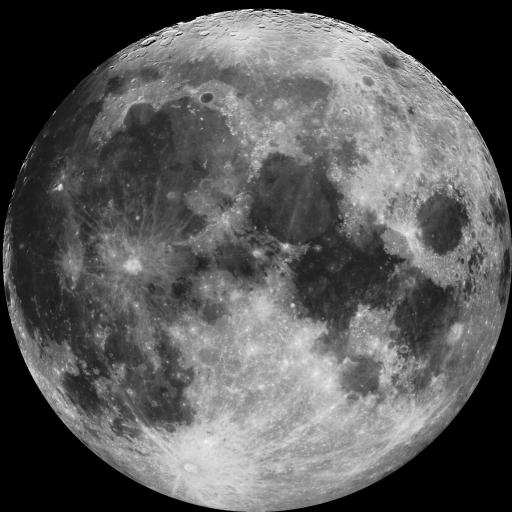
\includegraphics[width=0.2\textwidth]{moon.jpg}}}\) ~
    \tikz{\draw[-latex,mm2skyblue,thick] (0,0) -- node[above] {Degradation}
      (1.7,0);} ~
    \(\vcenter{\hbox{\includegraphics[width=0.2\textwidth]{figures/degraded_moon.jpg}}}\)
    ~
    \tikz{\draw[-latex,mm2skyblue,thick] (0,0) -- node[above] {Filtering}
      (1.7,0);} ~
    \(\vcenter{\hbox{\includegraphics[width=0.2\textwidth]{figures/filtered_moon.jpg}}}\)
    \caption{Picture of the Moon taken by the Galileo spacecraft on 7 December 1992}
  \end{figure}
\end{frame}

\begin{frame}
  \frametitle{The theory}
  Suppose you have a \alert{signal} \(S(\bm{t})\) in the time domain (whatever
  ``time'' is: actual time, point in space, pixel of an image, etc), degraded by
  \alert{known blurring shift-invariant function} \(B(\bm{t})\) and
  \alert{additive noise} \(N(\bm{t})\)
  \begin{equation*}
    X(\bm{t}) = (B * S)(\bm{t}) + N(\bm{t})
  \end{equation*}
  Its Fourier transform in the frequency domain is
  \begin{equation*}
    \hat{X}(\bm{f}) = \mathcal{F}(X)(\bm{f}) = \hat{B}(\bm{f})\hat{S}(\bm{f}) +
    \hat{N}(\bm{f})
  \end{equation*}
\end{frame}

\begin{frame}
  \frametitle{The theory (cont.)}
  We want to find an appropriate filter \(W(\bm{f})\) such that the function
  \(W(\bm{f})\hat{X}(\bm{f})\) is as much close as possible to the Fourier
  transform of the original signal \(\hat{S}(\bm{f}) = \mathcal{F}(S)(\bm{f})\),
  i.e. we want to minimize the quantity
  \begin{equation*}
    \Braket{W(\bm{f})\hat{X}(\bm{f}) - \hat{S}(\bm{f})} =
    \Braket{W(\bm{f})(\hat{B}(\bm{f})\hat{S}(\bm{f}) + \hat{N}(\bm{f})) -
      \hat{S}(\bm{f})}
  \end{equation*}
  This condition is fulfilled by
  \begin{equation*}
    W(\bm{f}) = \frac{\hat{B}^{*}(\bm{f})}{|\hat{B}(\bm{f})|^{2} +
      |\hat{N}(\bm{f})|^{2}/|\hat{S}(\bm{f})|^{2}}
  \end{equation*}
  This is the \alert{Wiener filter} function and
  \(\mathcal{F}^{-1}(W\hat{X})(\bm{t})\) is the \alert{filtered signal}.  This
  function gives more importance to frequencies with \alert{higher signal to
    noise ratio}.  In absence of blurring
  \begin{equation*}
    W(\bm{f}) = \frac{|\hat{S}(\bm{f})|^{2}}{|\hat{S}(\bm{f})|^{2} +
      |\hat{N}(\bm{f})|^{2}}
  \end{equation*}
\end{frame}

\begin{frame}
  \frametitle{The theory (cont.)}
  Theoretically, in order to calculate the Wiener filter function we need to
  know
  \begin{itemize}
  \item the original signal
  \item the blurring function
  \item the noise
  \end{itemize}
  or at least their power spectra.  Actually, power spectra need not to be known
  exactly (noise power spectrum can often be easily estimated, e.g. white noise
  has constant spectrum) because
  \begin{itemize}
  \item most signals of the same class have fairly similar power spectra
  \item the Wiener filter is insensitive to small variations in the original
    signal power spectrum
  \end{itemize}
  We can estimate the original signal power spectrum using a representative of
  the class of signals being filtered
\end{frame}

\begin{frame}
  \frametitle{Wiener filter applied to a temporal signal}
  IDL/GDL code:
  \lstinputlisting[linerange={13-35}]{filtro_wiener.pro}
\end{frame}

\begin{frame}
  \frametitle{Wiener filter applied to a temporal signal (cont.)}
  \begin{figure}
    \centering
    \includegraphics[width=0.85\textwidth]{figures/signal}
  \end{figure}
\end{frame}

\begin{frame}
  \frametitle{Wiener filter applied to a temporal signal (cont.)}
  \begin{figure}
    \centering
    \includegraphics[width=0.85\textwidth]{figures/signal-noise}
  \end{figure}
\end{frame}

\begin{frame}
  \frametitle{Wiener filter applied to a temporal signal (cont.)}
  \begin{figure}
    \centering
    \includegraphics[width=0.85\textwidth]{figures/result}
  \end{figure}
\end{frame}

\begin{frame}
  \frametitle{Wiener filter applied to an image}
  IDL/GDL code:
  \lstinputlisting[linerange={51-74}]{filtro_wiener.pro}
\end{frame}

\begin{frame}
  \frametitle{Wiener filter applied to an image (cont.)}
  \begin{figure}
    \centering
    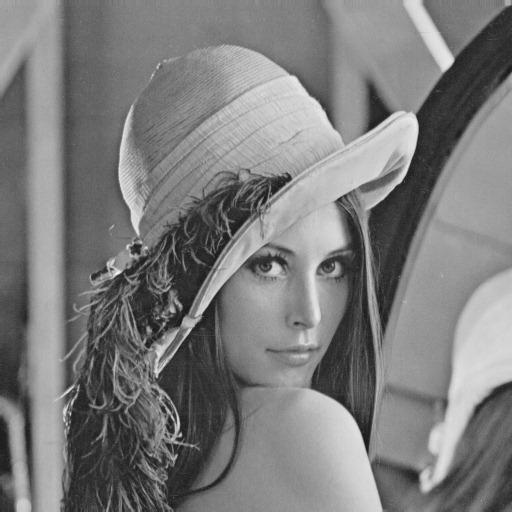
\includegraphics[width=0.55\textwidth]{lena}
    \caption{The original image, file \texttt{lena.jpg}}
  \end{figure}
\end{frame}

\begin{frame}
  \frametitle{Wiener filter applied to an image (cont.)}
  \begin{figure}
    \centering
    \includegraphics[width=0.55\textwidth]{figures/degraded_lena}
    \caption{The image has been degraded with a large noise}
  \end{figure}
\end{frame}

\begin{frame}
  \frametitle{Wiener filter applied to an image (cont.)}
  \begin{figure}
    \centering
    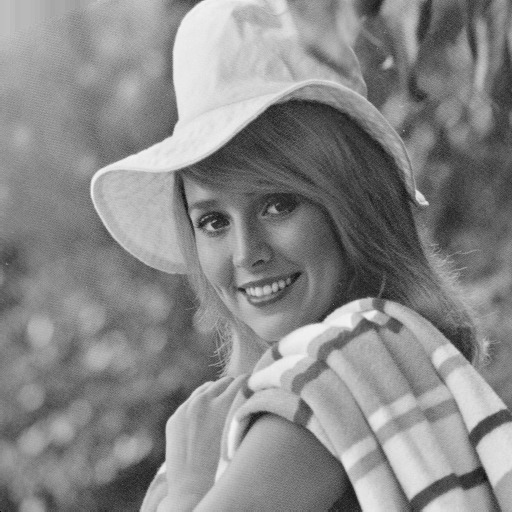
\includegraphics[width=0.55\textwidth]{elaine}
    \caption{The picture used to filter the degraded image, file
      \texttt{elaine.jpg}}
  \end{figure}
\end{frame}

\begin{frame}
  \frametitle{Wiener filter applied to an image (cont.)}
  We can use a different picture to filter the degraded image because they have
  similar power spectra
  \begin{figure}
    \centering
    \includegraphics[width=\textwidth]{figures/power-spectra}
    \caption{Left: power spectrum of \texttt{lena.jpg} file; right: power
      spectrum of \texttt{elaine.jpg} file}
  \end{figure}
\end{frame}

\begin{frame}
  \frametitle{Wiener filter applied to an image (cont.)}
  \begin{figure}
    \centering
    \includegraphics[width=0.55\textwidth]{figures/filtered_lena}
    \caption{The filtered image}
  \end{figure}
\end{frame}

\begin{frame}
  \frametitle{\refname}
  \nocite{*}
  \printbibliography{}
\end{frame}
\end{document}

%%% Local Variables:
%%% mode: latex
%%% TeX-master: t
%%% ispell-local-dictionary: "american"
%%% End:
